\documentclass[
	ngerman,
	toc=listof, % Abbildungsverzeichnis sowie Tabellenverzeichnis in das Inhaltsverzeichnis aufnehmen
	toc=bibliography, % Literaturverzeichnis in das Inhaltsverzeichnis aufnehmen
	footnotes=multiple, % Trennen von direkt aufeinander folgenden Fußnoten
	parskip=half, % vertikalen Abstand zwischen Absätzen verwenden anstatt horizontale Einrückung von Folgeabsätzen
	numbers=noendperiod % Den letzten Punkt nach einer Nummerierung entfernen (nach DIN 5008)
]{scrartcl}
\pdfminorversion=5 % erlaubt das Einfügen von pdf-Dateien bis Version 1.7, ohne eine Fehlermeldung zu werfen (keine Garantie für fehlerfreies Einbetten!)

% Dokumenteninformationen ----------------------------------------------------
\newcommand{\titel}{Architektur}
\newcommand{\untertitel}{Studienarbeit \semester}
\newcommand{\kompletterTitel}{\titel{} \\ \untertitel}
\newcommand{\datum}{\today}

\newcommand{\vorlagenOrdner}{../../99_Vorlagen} % Falls im Unterordner ../ vorne hinzufügen

\newcommand{\betriebLogo}{\vorlagenOrdner/Bilder/logo}

% Konfiguration -------------------------------------------------------------
\newcommand{\autoren}{
    \author{
        Schmid, Mike\\
        \texttt{sgschwin@hsr.ch}
        \and
        Schlatter, Janik\\
        \texttt{jschlatt@hsr.ch}
    }
}

\newcommand{\betreuer}{
    Stettler Beat\\
    \scriptsize \texttt{\url{beat.stettler@hsr.ch}}
    \normalsize
}

\newcommand{\schmid}{
    Mike Schmid\\
    \url{mschmid@hsr.ch}
    \normalsize
}

\newcommand{\schlatter}{
    Janik Schlatter\\
    \scriptsize \url{jschlatt@hsr.ch}
    \normalsize
}

\newcommand{\autorenNamen}{
    M. Schmid, J. Schlatter
}

\newcommand{\semester}{FS-2020}
\newcommand{\betriebName}{\textsc{HSR} Hochschule für Technik Rapperswil} % Metadaten zu diesem Dokument (Autor usw.)
% !TEX root = ../Projektdokumentation.tex

% Anpassung an Landessprache ---------------------------------------------------
\usepackage[english, main=ngerman]{babel} % \selectlanguage{english} if  needed

% Umlaute ----------------------------------------------------------------------
%   Umlaute/Sonderzeichen wie äüöß direkt im Quelltext verwenden (CodePage).
%   Erlaubt automatische Trennung von Worten mit Umlauten.
% ------------------------------------------------------------------------------
\usepackage[T1]{fontenc}
\usepackage[utf8]{inputenc}
\usepackage{textcomp} % Euro-Zeichen etc.

% Schrift ----------------------------------------------------------------------
\usepackage{lmodern} % bessere Fonts
\usepackage{relsize} % Schriftgröße relativ festlegen

% Tabellen ---------------------------------------------------------------------
\PassOptionsToPackage{table}{xcolor}
\usepackage{tabularx}
\usepackage{tabulary}
\usepackage{booktabs}
\usepackage{makecell}
\usepackage[table,xcdraw]{xcolor}
% für lange Tabellen
\usepackage{longtable}
\usepackage{array}
\usepackage{ragged2e}
\usepackage{lscape}
% Multi Columns
\usepackage{multicol}

% Grafiken ---------------------------------------------------------------------
\usepackage[dvips,final]{graphicx} % Einbinden von JPG-Grafiken ermöglichen
\usepackage{graphics} % keepaspectratio
\usepackage{floatflt} % zum Umfließen von Bildern
\graphicspath{{Bilder/}} % hier liegen die Bilder des Dokuments

% Sonstiges --------------------------------------------------------------------
\usepackage[titles]{tocloft} % Inhaltsverzeichnis DIN 5008 gerecht einrücken
\usepackage{enumitem} % anpassbare Enumerates/Itemizes
\usepackage{xspace} % sorgt dafür, dass Leerzeichen hinter parameterlosen Makros nicht als Makroendezeichen interpretiert werden

\usepackage{makeidx} % für Index-Ausgabe mit \printindex
\usepackage[printonlyused]{acronym} % es werden nur benutzte Definitionen aufgelistet

% Einfache Definition der Zeilenabstände und Seitenränder etc.
\usepackage{setspace}
\usepackage{geometry}

% Symbolverzeichnis
\usepackage[intoc]{nomencl}
\let\abbrev\nomenclature
\renewcommand{\nomname}{Abkürzungsverzeichnis}
\setlength{\nomlabelwidth}{.25\hsize}
\renewcommand{\nomlabel}[1]{#1 \dotfill}
\setlength{\nomitemsep}{-\parsep}

\usepackage{varioref} % Elegantere Verweise. „auf der nächsten Seite“
\usepackage{url} % URL verlinken, lange URLs umbrechen etc.

\usepackage{chngcntr} % fortlaufendes Durchnummerieren der Fußnoten
% \usepackage[perpage]{footmisc} % Alternative: Nummerierung der Fußnoten auf jeder Seite neu

\usepackage{ifthen} % bei der Definition eigener Befehle benötigt
\usepackage{todonotes} % definiert u.a. die Befehle \todo und \listoftodos
\usepackage[square]{natbib} % wichtig für korrekte Zitierweise

% PDF-Optionen -----------------------------------------------------------------
\usepackage{pdfpages}
\pdfminorversion=5 % erlaubt das Einfügen von pdf-Dateien bis Version 1.7, ohne eine Fehlermeldung zu werfen (keine Garantie für fehlerfreies Einbetten!)
\usepackage[
    bookmarks,
    bookmarksnumbered,
    bookmarksopen=true,
    bookmarksopenlevel=1,
    colorlinks=true,
% diese Farbdefinitionen zeichnen Links im PDF farblich aus
    linkcolor=AOBlau, % einfache interne Verknüpfungen
    anchorcolor=AOBlau,% Ankertext
    citecolor=AOBlau, % Verweise auf Literaturverzeichniseinträge im Text
    filecolor=AOBlau, % Verknüpfungen, die lokale Dateien öffnen
    menucolor=AOBlau, % Acrobat-Menüpunkte
    urlcolor=AOBlau,
% diese Farbdefinitionen sollten für den Druck verwendet werden (alles schwarz)
    %linkcolor=black, % einfache interne Verknüpfungen
    %anchorcolor=black, % Ankertext
    %citecolor=black, % Verweise auf Literaturverzeichniseinträge im Text
    %filecolor=black, % Verknüpfungen, die lokale Dateien öffnen
    %menucolor=black, % Acrobat-Menüpunkte
    %urlcolor=black,
%
    %backref, % Quellen werden zurück auf ihre Zitate verlinkt
    pdftex,
    plainpages=false, % zur korrekten Erstellung der Bookmarks
    pdfpagelabels=true, % zur korrekten Erstellung der Bookmarks
    hypertexnames=false, % zur korrekten Erstellung der Bookmarks
    linktocpage % Seitenzahlen anstatt Text im Inhaltsverzeichnis verlinken
]{hyperref}
% Befehle, die Umlaute ausgeben, führen zu Fehlern, wenn sie hyperref als Optionen übergeben werden
\hypersetup{
    pdftitle={\titel -- \untertitel},
    pdfauthor={\autoren},
    pdfcreator={\autoren},
    pdfsubject={\titel -- \untertitel},
    pdfkeywords={\titel -- \untertitel},
}


% zum Einbinden von Programmcode -----------------------------------------------
\usepackage{listings}
\usepackage{xcolor}
\usepackage{beramono}
% Pseudocode
\usepackage{algorithmic}
\usepackage[linesnumbered,ruled]{algorithm2e}

\definecolor{hellgelb}{rgb}{1,1,0.9}
\definecolor{colKeys}{rgb}{0,0,1}
\definecolor{colIdentifier}{rgb}{0,0,0}
\definecolor{colComments}{rgb}{0,0.5,0}
\definecolor{colString}{rgb}{1,0,0}
\definecolor{bluekeywords}{rgb}{0,0,1}
\definecolor{greencomments}{rgb}{0,0.5,0}
\definecolor{redstrings}{rgb}{0.64,0.08,0.08}
\definecolor{xmlcomments}{rgb}{0.5,0.5,0.5}
\definecolor{types}{rgb}{0.17,0.57,0.68}
\definecolor{DarkPurple}{rgb}{0.4, 0.1, 0.4}
\definecolor{DarkCyan}{rgb}{0.0, 0.5, 0.4}
\definecolor{LightLime}{rgb}{0.3, 0.5, 0.4}
\definecolor{Blue}{rgb}{0.0, 0.0, 1.0}
\definecolor{AOBlau}{rgb}{0, 0.28, 0.56}
% Tabellenfärbung:
\definecolor{heading}{rgb}{0.64,0.78,0.86}
\definecolor{odd}{rgb}{0.9,0.9,0.9}

\lstset{
    float=hbp,
	basicstyle=\footnotesize,
    identifierstyle=\color{colIdentifier},
    keywordstyle=\color{colKeys},
    stringstyle=\color{colString},
    commentstyle=\color{colComments},
    backgroundcolor=\color{hellgelb},
    columns=flexible,
    tabsize=2,
    frame=single,
    extendedchars=true,
    showspaces=false,
    showstringspaces=false,
    numbers=left,
    numberstyle=\tiny,
    breaklines=true,
    breakautoindent=true,
	captionpos=b,
}
\lstdefinestyle{visual-studio-style}{
	language=[Sharp]C,
	columns=flexible,
	showstringspaces=false,
	basicstyle=\footnotesize\ttfamily, 
	commentstyle=\color{greencomments},
	morekeywords={partial, var, value, get, set},
	keywordstyle=\bfseries\color{bluekeywords},
	stringstyle=\color{redstrings},
	breaklines=true,
	breakatwhitespace=true,
	tabsize=4,
	numbers=left,
	numberstyle=\tiny\color{black},
	frame=lines,
	showspaces=false,
	showtabs=false,
	escapeinside={£}{£},
}
\lstdefinestyle{eclipse-style}{
	language=Java,  
	columns=flexible,
	showstringspaces=false,     
	basicstyle=\footnotesize\ttfamily, 
	keywordstyle=\bfseries\color{DarkPurple},
	commentstyle=\color{LightLime},
	stringstyle=\color{Blue}, 
	escapeinside={£}{£}, % latex scope within code      
	breaklines=true,
	breakatwhitespace=true,
	showspaces=false,
	showtabs=false,
	tabsize=4,
	morekeywords={length},
	numbers=left,
	numberstyle=\tiny\color{black},
	frame=lines,
}
\lstset{style=eclipse-style}
\lstdefinelanguage{cs}{
	sensitive=false,
	morecomment=[l]{//},
	morecomment=[s]{/*}{*/},
	morestring=[b]",
	morekeywords={
		abstract,event,new,struct,as,explicit,null,switch
		base,extern,object,this,bool,false,operator,throw,
		break,finally,out,true,byte,fixed,override,try,
		case,float,params,typeof,catch,for,private,uint,
		char,foreach,protected,ulong,checked,goto,public,unchecked,
		class,if,readonly,unsafe,const,implicit,ref,ushort,
		continue,in,return,using,decimal,int,sbyte,virtual,
		default,interface,sealed,volatile,delegate,internal,short,void,
		do,is,sizeof,while,double,lock,stackalloc,
		else,long,static,enum,namespace,string},
}
\lstdefinelanguage{natural}{
	sensitive=false,
	morecomment=[l]{/*},
	morestring=[b]",
	morestring=[b]',
	alsodigit={-,*},
	morekeywords={
		DEFINE,DATA,LOCAL,END-DEFINE,WRITE,CALLNAT,PARAMETER,USING,
		IF,NOT,END-IF,ON,*ERROR-NR,ERROR,END-ERROR,ESCAPE,ROUTINE,
		PERFORM,SUBROUTINE,END-SUBROUTINE,CONST,END-FOR,END,FOR,RESIZE,
		ARRAY,TO,BY,VALUE,RESET,COMPRESS,INTO,EQ},
}
\lstdefinelanguage{php}{
	sensitive=false,
	morecomment=[l]{/*},
	morestring=[b]",
	morestring=[b]',
	alsodigit={-,*},
	morekeywords={
		abstract,and,array,as,break,case,catch,cfunction,class,clone,const,
		continue,declare,default,do,else,elseif,enddeclare,endfor,endforeach,
		endif,endswitch,endwhile,extends,final,for,foreach,function,global,
		goto,if,implements,interface,instanceof,namespace,new,old_function,or,
		private,protected,public,static,switch,throw,try,use,var,while,xor
		die,echo,empty,exit,eval,include,include_once,isset,list,require,
		require_once,return,print,unset},
}
 % verwendete Packages
% !TEX root = ../Projektdokumentation.tex

% Seitenränder -----------------------------------------------------------------
\setlength{\topskip}{\ht\strutbox} % behebt Warnung von geometry
\geometry{
	a4paper,
	left=20mm,
	right=20mm,
	top=25mm,
	bottom=40mm
}

\usepackage[
	automark, % Kapitelangaben in Kopfzeile automatisch erstellen
	headsepline, % Trennlinie unter Kopfzeile
	% footsepline, % Trennlinie oberhalb Fusszeile
	ilines % Trennlinie linksbündig ausrichten
]{scrpage2}

% Kopf- und Fußzeilen ----------------------------------------------------------
\pagestyle{scrheadings}
% chapterpagestyle gibt es nicht in scrartcl
%\renewcommand{\chapterpagestyle}{scrheadings}
\clearscrheadfoot

% Kopfzeile
\renewcommand{\headfont}{\normalfont} % Schriftform der Kopfzeile
\ihead{\large{\textsc{\titel}}\\ \small{\untertitel} \\[2ex] \textit{\headmark}}
\chead{}
%\ohead{\includegraphics[scale=0.125]{\betriebLogo}}
\setlength{\headheight}{20mm} % Höhe der Kopfzeile
%\setheadwidth[0pt]{textwithmarginpar} % Kopfzeile über den Text hinaus verbreitern (falls Logo den Text überdeckt)

% Fußzeile
\ifoot{\autorenNamen}
\cfoot{}
\ofoot{\pagemark}

% Überschriften nach DIN 5008 in einer Fluchtlinie
% ------------------------------------------------------------------------------

% Abstand zwischen Nummerierung und Überschrift definieren
% > Schön wäre hier die dynamische Berechnung des Abstandes in Abhängigkeit
% > der Verschachtelungstiefe des Inhaltsverzeichnisses
\newcommand{\headingSpace}{1.5cm}

% Abschnittsüberschriften im selben Stil wie beim Inhaltsverzeichnis einrücken
\renewcommand*{\othersectionlevelsformat}[3]{
  \makebox[\headingSpace][l]{#3\autodot}
}

% Für die Einrückung wird das Paket tocloft benötigt
%\cftsetindents{chapter}{0.0cm}{\headingSpace}
\cftsetindents{section}{0.0cm}{\headingSpace}
\cftsetindents{subsection}{0.0cm}{\headingSpace}
\cftsetindents{subsubsection}{0.0cm}{\headingSpace}
\cftsetindents{figure}{0.0cm}{\headingSpace}
\cftsetindents{table}{0.0cm}{\headingSpace}

% Allgemeines
% ------------------------------------------------------------------------------

\onehalfspacing % Zeilenabstand 1,5 Zeilen
\frenchspacing % erzeugt ein wenig mehr Platz hinter einem Punkt

% Schusterjungen und Hurenkinder vermeiden
\clubpenalty = 10000
\widowpenalty = 10000
\displaywidowpenalty = 10000

% Quellcode-Ausgabe formatieren
\lstset{numbers=left, numberstyle=\tiny, numbersep=5pt, breaklines=true}
\lstset{emph={square}, emphstyle=\color{red}, emph={[2]root,base}, emphstyle={[2]\color{blue}}}

\counterwithout{footnote}{section} % Fußnoten fortlaufend durchnummerieren
\setcounter{tocdepth}{\subsubsectionlevel} % im Inhaltsverzeichnis werden die Kapitel bis zum Level der subsubsection übernommen
\setcounter{secnumdepth}{\subsubsectionlevel} % Kapitel bis zum Level der subsubsection werden nummeriert

% Aufzählungen anpassen
\renewcommand{\labelenumi}{\arabic{enumi}.}
\renewcommand{\labelenumii}{\arabic{enumi}.\arabic{enumii}.}
\renewcommand{\labelenumiii}{\arabic{enumi}.\arabic{enumii}.\arabic{enumiii}}
 % Definitionen zum Aussehen der Seiten
% !TEX root = ../Projektdokumentation.tex

% Abkürzungen, ggfs. mit korrektem Leerraum
\newcommand{\bs}{$\backslash$\xspace}
\newcommand{\bspw}{bspw.\xspace}
\newcommand{\bzw}{bzw.\xspace}
\newcommand{\ca}{ca.\xspace}
\newcommand{\dahe}{\mbox{d.\,h.}\xspace}
\newcommand{\etc}{etc.\xspace}
\newcommand{\eur}[1]{\mbox{#1\,\texteuro}\xspace}
\newcommand{\evtl}{evtl.\xspace}
\newcommand{\ggfs}{ggfs.\xspace}
\newcommand{\Ggfs}{Ggfs.\xspace}
\newcommand{\gqq}[1]{\glqq{}#1\grqq{}}
\newcommand{\inkl}{inkl.\xspace}
\newcommand{\insb}{insb.\xspace}
\newcommand{\ua}{\mbox{u.\,a.}\xspace}
\newcommand{\usw}{usw.\xspace}
\newcommand{\Vgl}{Vgl.\xspace}
\newcommand{\zB}{\mbox{z.\,B.}\xspace}

% Befehle für häufig anfallende Aufgaben
\newcommand{\Abbildung}[1]{\autoref{fig:#1}}
\newcommand{\Anhang}[1]{\appendixname{}~\ref{#1}: \nameref{#1} \vpageref{#1}}
\newcommand{\includegraphicsKeepAspectRatio}[2]{\includegraphics[width=#2\textwidth,height=#2\textheight,keepaspectratio]{#1}}
\newcommand{\Zitat}[2][\empty]{\ifthenelse{\equal{#1}{\empty}}{\citep{#2}}{\citep[#1]{#2}}}
\newcommand{\Autor}[1]{\textsc{#1}} % zum Ausgeben von Autoren
\newcommand{\itemd}[2]{\item{\textbf{#1}}\\{#2}} % erzeugt ein Listenelement mit fetter Überschrift

% einfaches Wechseln der Schrift, z.B.: \changefont{cmss}{sbc}{n}
\newcommand{\changefont}[3]{\fontfamily{#1} \fontseries{#2} \fontshape{#3} \selectfont}

% Verwendung analog zu \includegraphics
\newlength{\myx} % Variable zum Speichern der Bildbreite
\newlength{\myy} % Variable zum Speichern der Bildhöhe
\newcommand\includegraphicstotab[2][\relax]{%
% Abspeichern der Bildabmessungen
\settowidth{\myx}{\includegraphics[{#1}]{#2}}%
\settoheight{\myy}{\includegraphics[{#1}]{#2}}%
% das eigentliche Einfügen
\parbox[c][1.1\myy][c]{\myx}{%
\includegraphics[{#1}]{#2}}%
}

% verschiedene Befehle um Wörter semantisch auszuzeichnen ----------------------
\newcommand{\Index}[2][\empty]{\ifthenelse{\equal{#1}{\empty}}{\index{#2}#2}{\index{#1}#2}}
\newcommand{\Fachbegriff}[2][\empty]{\ifthenelse{\equal{#1}{\empty}}{\textit{\Index{#2}}}{\textit{\Index[#1]{#2}}}}
\newcommand{\NeuerBegriff}[2][\empty]{\ifthenelse{\equal{#1}{\empty}}{\textbf{\Index{#2}}}{\textbf{\Index[#1]{#2}}}}

\newcommand{\Ausgabe}[1]{\texttt{#1}}
\newcommand{\Eingabe}[1]{\texttt{#1}}
\newcommand{\Code}[1]{\texttt{#1}}
\newcommand{\Datei}[1]{\texttt{#1}}

\newcommand{\Assembly}[1]{\textsf{#1}}
\newcommand{\Klasse}[1]{\textsf{#1}}
\newcommand{\Methode}[1]{\textsf{#1}}
\newcommand{\Attribut}[1]{\textsf{#1}}

\newcommand{\Datentyp}[1]{\textsf{#1}}
\newcommand{\XMLElement}[1]{\textsf{#1}}
\newcommand{\Webservice}[1]{\textsf{#1}}

\newcommand{\Refactoring}[1]{\Fachbegriff{#1}}
\newcommand{\CodeSmell}[1]{\Fachbegriff{#1}}
\newcommand{\Metrik}[1]{\Fachbegriff{#1}}
\newcommand{\DesignPattern}[1]{\Fachbegriff{#1}}

\newcommand{\muss}[1]{\textcolor{red}{#1}}
\newcommand{\soll}[1]{\textcolor{orange}{#1}}
\newcommand{\kann}[1]{\textcolor{blue}{#1}}

\newcommand{\success}[1]{\textcolor{greencomments}{#1}}
\newcommand{\fail}[1]{\textcolor{red}{#1}} % eigene allgemeine Befehle, die z.B. die Arbeit mit LaTeX erleichtern

\begin{document}

% Deckblatt ------------------------------------------------------------------
\phantomsection
\thispagestyle{plain}
\pdfbookmark[1]{Deckblatt}{deckblatt}
\begin{titlepage}
    \begin{center}
        \includegraphics[scale=1.5]{\betriebLogo}\\[10ex]

        \rule{\linewidth}{0.5mm}\\[2ex]
        {\huge \bfseries  \titel }\\[2ex]
        {\LARGE \untertitel }\\[2ex]
        {\large \datum}\\
        \rule{\linewidth}{0.5mm}\\[10ex]

        \begin{minipage}[t]{0.4\textwidth}
            \begin{flushleft} 
                \large \emph{Autoren:}\\
                    \large Mike \textsc{Schmid}\\
                    \scriptsize \texttt{mike.schmid@hsr.ch}\\[1ex]
                    \large Janik \textsc{Schlatter}\\
                    \scriptsize \texttt{janik.schlatter@hsr.ch}\\[1ex]
            \end{flushleft}
            \end{minipage}
            ~
            \begin{minipage}[t]{0.4\textwidth}
            \begin{flushright} 
                \large \emph{Supervisor:} \\
                Prof. Stettler \textsc{Beat}\\
                \scriptsize \texttt{beat.stettler@hsr.ch}\\[1ex]
            \end{flushright}
        \end{minipage}\\[40ex]

        \small
        \noindent
        Dieses Werk einschließlich seiner Teile ist \textbf{urheberrechtlich geschützt}.
        Jede Verwertung außerhalb der engen Grenzen des Urheberrechtgesetzes ist ohne
        Zustimmung des Autors unzulässig und strafbar. Das gilt insbesondere für
        Vervielfältigungen, Übersetzungen, Mikroverfilmungen sowie die Einspeicherung
        und Verarbeitung in elektronischen Systemen.

    \end{center}
\end{titlepage}
\cleardoublepage

% Preface --------------------------------------------------------------------
\pagenumbering{Roman}

% Zweck
\section*{Zweck}
Dieses Dokument beschreibt die Architektur, die Möglichkeiten für die Auswahl der Technolodien und die Entscheidungen zum Design und der Architektur des Projektes.

% Änderungsgeschichte
\section*{Änderungsgeschichte}
\begin{tabularx}{\textwidth}{llXl}
	\toprule
	Datum & Version & Änderung & Autor \\
	\midrule
	24.03.2018 & 1.0 & Initial Setup & Janik Schlatter \\
	26.03.2020 & 1.0 & Designentscheidungen & Mike Schmid \\ 
	02.04.2020 & 1.1 & Anpassungen gem. Besprechung vom 01.04.2020 & Mike Schmid \\
	\bottomrule
\end{tabularx}
\cleardoublepage

% Inhaltsverzeichnis
\phantomsection
\pdfbookmark[1]{Inhaltsverzeichnis}{inhalt}
\tableofcontents
\cleardoublepage

\pagenumbering{arabic}
% Jede Überschrift 1 auf neuer Seite
\let\stdsection\section
\renewcommand\section{\clearpage\stdsection}

% Inhalt ---------------------------------------------------------------------
\section{Designentscheidungen}
	\subsection{Architekturentscheidungen}
		\subsubsection{Anwendung von Patterns}
		Patterns in der Softwareentwicklung sind Vorschläge, wie mit bekannten Problemen umgegangen werden soll.
		Verschiedene Patterns können auf unterschiedliche Probleme angewandt werden und helfen, verschiedene Probleme zu lösen.
		Es gibt eine Vielfalt von Patterns mit vielen Anwendungsmöglichkeiten und Kombinationen.
		Für das Zu entwickelnde System wurden zwei Patterns ausgewählt, die die Erweiterbarkeit gewährleisten sollen.

		\paragraph{Entscheidung 1: Anwendung von Patterns für die Testerstellung}
		\begin{itemize}
			\item Im Kontext der Erweiterbarkeit des zu entwickelnden Systems,
			\item damit weitere Netzwerktest einfach hinzugefügt werden können,
			\item wurde entschieden, dass für die Testerstellung das Strategy und Factory-Method Pattern angewandt wird,
			\item um die Instanzierungslogik von den einzelnen Testklassen zu entkoppeln.
			\item Dabei wird akzeptiert, dass die Implementation des Systems alles in allem komplexer, und die Erstellung umfangreicher wird.			
		\end{itemize}

		\paragraph{Entscheidung 2: Anwendung von Patterns für die Kommunikationsschnittstellen}
		\begin{itemize}
			\item Im Kontext der Erweiterbarkeit um weitere Netzwerkschnittstellen,
			\item damit das Hinzufügen von weiteren Schnittstellen vereinfacht wird,
			\item wurde entschieden, dass die Auswahl und Instanzierung von Verbindungen über ein Factory Method- und Strategy Pattern realisiert wird.
			\item um die Verbindungsauswahl vom System zu entkoppeln.
			\item Es wird dabei akzeptiert, dass das System komplexer wird und die Erstellung mehr Aufwand benötigt.
		\end{itemize}

		Das Strategy Pattern ist ein Verhaltenspattern und ermöglicht eine erhöhte Austauschbarkeit einzelner Softwarekomponenten.
		Eine gruppe von Algorithmen wird zu einer Strategie zusammengefasst und können untereinander leicht ausgetauscht werden.
		
		Das Factory Method Pattern erlaubt die instanzierung von Objekten, ohne die spezifische Klasse des Objekts kennen zu müssen.
		Somit wird die Flexibilität der Software und die Austauschbarkeit der einzelnen Komponenten erhöht.
		
		Weitere Software-Pattern werden im Verlauf der Arbeit bei Bedarf verwendet, sind aber nicht Teil der Architekturentscheidungen.
		\newpage

		\subsubsection{Testdefinitionssprache}
		Die Testdefinitionen benötigen ein einheitliches Format, damit sie vom Programm interpretiert werden können und dass daraus Tests erstellt werden können.
		Für diese Aufgabe gibt es eine Vielzahl von verschiedenen Beschreibungssprachen.
		
		XML (Extensible Markup Language) ist eine Auszeichnungssprache, die in der Informatik oft angewandt wird, wenn Daten in einer Hierarchischen Struktur in einer Textdatei beschrieben werden.
		Der grösste Vorteil in der Verwendung von XML ist die hohe Verbreitung und Platformunabhängigkeit.
		Nachteile sind eine höhere Redundanz als in anderen Formaten was zu höherem Speicherverbrauch und grösserem Bandbreitenverwendung führt, wenn Daten im XML-Format gespeichert oder über das Internet versendet werden.

		JSON (Javascript Object Notation) ist Menschenlesbar, Leichtgewichtig und wird zum effizienten Austausch von Informationen in einem geordneten Format auszutauschen.
		Das Format baut auf einer Attribut : Attributwert Logik auf und ist im Vergleich zu XML effizienter über das Internet austauschbar.
		Im Gegensatz zu XML bietet JSON aber keine Schemas, ein einheitliches Format für den Datenaustausch, was die Verwendung in verschiedenen Systemen komplizierter macht.

		YAML (YAML ain't Markup Language) ist ein Datenserialisierungsformat mit Fokus auf Menschenlesbarkeit und wird hauptsächlich für die Erstellung von Konfigurationsdaten verwendet.
		Die grössten Vorteile sind die Datenkonsistenz der Datenmodel und die hohe Portierbarkeit zwischen verschiedensten Programmiersprachen.
		Zu den Nachteilen gehört die geringere Performanz gegenüber XML und JSON und die geringere Verbreitung von YAML.
		Ein weiterer Wichtiger Punkt ist, dass Netzwerktechniker in der Lage sein sollten, YAML zu lesen und schreiben.

		\paragraph{Entscheidung 3: Auswahl der Testdefinitionssprache}
		\begin{itemize}
			\item Um die Testdefinitionen in einer möglichst menschenlesbaren Form zu halten,
			\item und die Verwendbarkeit im zu entwickelnden System zu gewährleisten,
			\item haben wir entschieden, die Testdefinitionen in YAML zu verfassen,
			\item um ein Format zu verwenden, dass auch von Netzwerkleuten verwendet wird.
			\item Andere Technologien, wie JSON, XML usw. werden dabei voraussichtlich weggelassen,
			\item auch wenn diese in spezifischen Anwendungen wie die Speicherung von Daten geeignet wären.
		\end{itemize}
		\newpage

		\subsubsection{Benutzeroberfläche}
		Damit Benutzer des Systems mit diesem interagieren können, wird eine Benutzeroberfläche benötigt.
		Das Design der Oberfläche spielt eine entscheidende Rolle für die Benutzbarkeit der Software. 
		Mögliche Umsetzungen sind eine Grafische Benutzeroberfläche (GUI), die es Benutzern erlaubt über eine vordefinierte Oberfläche mit dem Programm zu interagieren.
		Weiterhin lässt sich das System auch mit einem Kommandozeilen-Userinterface umsetzen, welches weitaus einfacher in der Implementation ist, aber gegenüber dem GUI weniger Interaktionsmöglichkeiten bietet.

		\paragraph{Entscheidung 4: Weglassen einer Grafischen Benutzeroberfläche}
		\begin{itemize}
			\item Im Rahmen der zeitlichen Beschränkung der Arbeit,
			\item um uns auf die Implementation der Logik zu konzentrieren,
			\item werden wir kein GUI entwickeln.
			\item Stattdessen wird, wo nötig, eine Kommandozeileninteraktion implementiert.
			\item Es wird akzeptiert, dass die Benutzerfreundlichkeit des zu entwickelnden Systems dadurch eingeschränkt wird.
		\end{itemize}

		\newpage

		\subsubsection{Testframework}
		Für die Kommunikation und das automatisierte Testen von Netzwerken gibt es verschiedene Möglichkeiten.
		Nachfolgend sind einige davon aufgelistet:
		
		Ansible ist ein Framework für automatisierte Netzwerkoperationen wie Konfiguration, Skalierung oder Testing.
		Das Framework arbeitet, ohne dass auf dem Zielgerät etwas installiert werden muss, das mit der Software kommuniziert, solange das Zielgerät über SSH erreichbar ist.
		Ansible ist vergleichsweise einfach zu erlernen und in Python geschrieben.
		Die Netzwerkkonfiguration wird im YAML Format erfasst und das Programm sorgt dafür, dass die gewünschte Konfiguration im Netzwerk umgesetzt wird.
		Nachteile sind der geringe Windows-Support und das fehlende Auflösen von Abhängigkeiten.

		Saltstack ist ein Konfigurations-Management-Framework mit Funktionen für automatische Neztwerktests.
		Parallele Programmausführung, Skalierbarkeit und eine aktive Community gehören zu den grössten Vorteilen.
		Allerdings ist der Installationsprozess für Neueinsteiger eher komplex und ausser für Linux ist der Betriebssystemsupport limitiert.
		Auch Saltstack ist in Python geschrieben, was die Erweiterbarkeit erhöht.
		
		Puppet ist eine konfigurationsautomatisierungs- und Deployment-organisations-Lösung für verteilte Software und Infrastruktur.
		Geschrieben in Ruby, bietet Puppet eine Vielzahl von Funktionen für die Orchestrierung, Konfigurationsautomatisierung, Visualisierung und Reporting.
		Stärken sind der Support für eine Vielzahl von Betriebssystemen, hohe Stabilität und Robustheit.
		Schwierigkeiten können die hohe Anfängerschwierigkeit, schwächere Skalierbarkeit und Flexibilität (verglichen mit den anderen Lösungen).

		Chef war ursprünglich ein Tool für internes End-zu-End Server Deployment und wurde später als Open Source Lösung für Cloud und Infrastruktur Automatisierung veröffentlicht.
		Es wird als eine der flexibelsten Lösungen für OS und Middleware Management beschrieben und wurde für Programmierer entwickelt.
		Chef hat eine ausführliche Dokumentation und ist sehr stabil und verlässlich für grosse Systeme.
		Die grössten Nachteile sind die steile Lernkurve und ein komplizierteres Inbetriebnehmen gegenüber den anderen Systemen.

		Nornir wurde in der Studienarbeit von Anfang an als mögliche Lösung für die Testautomation genannt.
		Das Framework wurde in Python für die Verwendung mit Python entwickelt und bietet eine Vielzahl von Möglichkeiten für die Ausführung von Tests auf verschiedensten Systemen.
		Nornir führt die Tests als serielle oder parallele Tasks aus und verwendet YAML für die Datenverwaltung.
		Allerdings lässt sich Nornir nicht einfach ausführen, sondern muss in ein Python-Programms implementiert werden.
		Deshalb kann Nornir nicht einfach Installiert und danach verwendet werden, sondern ist ein Tool, welches es erlaubt, eigene Netzwerktasks zu definieren und auszuführen.



		\paragraph{Entscheidung 5: Verwendung von Nornir als Testframework}
		\begin{itemize}
			\item Für die Kommunikation mit verschiedenen Netzwerken,
			\item um die Implementation möglichst zu vereinfachen,
			\item wurde entschieden, dass das System das Nornir-Automations-Framework verwendet wird,
			\item weil Nornir dafür gedacht ist, in einem Python-Programm eingesetzt zu werden
			\item und eine umfangreiche Sammlung von nützlichen Funktionen bietet, mit denen man Netzwerktests ausführen kann.
		\end{itemize}

		Die gesamte Arbeit wurde von Anfang an darauf ausgelegt, mit Nornir als Automatisierunsframework zu arbeiten.
		Die Vielseitigen Methoden, um mit Netzwerkgeräten zu kommunizieren und die Vielzahl von möglichen Befehlen erlauben es, einfachen und effizienten Code zu schreiben, welcher die Netzwerke testet.
		\newpage

		\subsubsection{Datenhaltung}
		Für die Verwaltung von Daten, insbesondere das persistente Speichern und Laden, gibt es diverse Möglichkeiten.
		Da die Testdefinitionen in YAML verfasst werden, wäre für die Verwaltung der YAML-Files ein0e Dokumentdatenbank geeignet.
		Dokumentdatenbanken entspringen aus dem NoSQL Paradigma und haben kein fixes definiertes Schema, was eine flexiblere Verwendung ermöglicht, aber auch Fehleranfälliger ist.
		Üblicherweise werden Dokumentdatenbanken in einem Key-Value Format gehalten, was die Verwendung mit YAML vereinfacht.

		Weiterhin liesse sich eine Relationale Datenbank implementieren, wobei dafür ein Datenbankschema entworfen werden müsste.
		Die Verwendung einer SQL-Datenbank würde zu einer stärkeren Konsistenz der Daten führen, da die Datenbank eine strenge Konsistenz erzwingt.
		Allerdings sind relationale Datenbanken im Vergleich zu NoSQL Datenbanken komplexer und lassen sich schwieriger Skalieren.

		Eine weitere Möglichkeit für die Speicherung der Daten wäre eine Graphdatenbank. Graphdatenbanken speichern nicht nur die Daten in Form von Knoten, sondern auch die Beziehungen zwischen den Daten in Form von Kanten zwischen den Knoten.
		Graphalgorithmen erlauben es, sehr effiziente Abfragen auf die Daten auszuführen und Verknüpfungen zwischen den Daten abzufragen, für die eine Relationale Datenbank viel komplexere und langsamere Queries verwenden würde.

		Ausserdem besteht noch die Möglichkeit, keine Datenbank zu implementieren und die Daten auf dem Clientsystem zu verwalten.
		Hierbei werden die YAML-Dokumente direkt auf der Dateiablage des Clients gespeichert. 
		Der Ansatz ist definitiv simpler als die Verwendung einer Datenbank, allerdings kann dies dazu führen, dass Konsistenzprobleme auftreten.
		Die Anwendung ohne Datenbank legt somit mehr Verantwortung in die Hände der Benutzer, welche sich selber darum kümmern müssen, dass die Daten in der richtigen Form persistent gespeichert werden.
		Es ist trotzdem möglich, gemeinsam einen Datensatz zu halten, beispielsweise liesse sich die Testkonfiguration über ein Git-Repository verwalten und von verschiedenen Standorten her verwenden.
		Auch die Verwendung mit einem zentralen Filesystem, z.B. ein Ordner auf dem Server ist grundsätzlich möglich, erfordert aber geringfügige Anpassungen am Programm, damit die Pfade korrekt verwendet werden.

		\paragraph{Entscheidung 6: Verzicht auf eine Datenbank}
		\begin{itemize}
			\item Um Daten persistent zu speichern, 
			\item damit sie vom System wieder abgerufen werden können,
			\item werden die Daten im YAML-Format abgelegt,
			\item und nicht in einer Datenbank,
			\item wobei ein Datenbanksystem für die zentralisierte Speicherung möglicherweise besser geeignet wäre.
		\end{itemize}
		\newpage

		\subsubsection{Deployment}
		Die fertige Software muss auf verschiedenen Systemen mit unterschiedlichen Betriebssystemen einsetzbar sein.
		Die Installation soll dabei so einfach wie möglich sein und eine geringe Anzahl Abhängigkeiten an weitere Software haben.
		Wenn das Programm beispielsweise fünf weitere Programme benötigt, die alle parallel dazu installiert werden müssen, könnte das für Netzwerktechniker ein Grund sein, eine andere Software zu wählen.
		Ausserdem führt eine kompliziertere Installation dazu, dass der Einstieg für Unerfahrene Netzwerkleute schwieriger wird.
		Somit sollte die Auslieferung möglichst simpel erfolgen und geringe/keine Abhängigkeiten haben.
		
		Eine Auslieferung als ausführbare Datei, z.B. im .Exe-Format für Windows-Benutzer, wäre sicher für die Benutzung am einfachsten,
		allerdings wäre das Programm dann nicht so einfach erweiterbar, weil für jede Änderung das Programm nochmals aktualisiert werden müsste.

		Das Deployment als Dockercontainer ist, unabhängig der eigentlichen Auslieferung, auch eine mögliche Option.
		Diese Möglichkeit hat aber mehr Abhängigkeiten gegenüber einer einfachen ausführbaren Datei, da auf dem Client-Computer zuerst noch Docker installiert werden muss.
		
		Die einfachste Variante ist die Auslieferung als reines Python-Skript. Der grösste Vorteil ist, dass sich ein Python Skript auf jedem System ausführen lässt, welches Python installiert hat.
		Die meisten Betriebssysteme haben heute per Default Python vorinstalliert, zumindest auf MacOS und Linux-Systemen.
		Somit liesse sich die Software, ohne weitere Software (ausser evtl Python) installieren zu müssen, verwenden.

		\paragraph{Entscheidung 7: Deployment als Python-Skript}
		\begin{itemize}
			\item Im Kontext des Deployments, der Auslieferung der Software,
			\item um das Programm auf möglichst vielen Plattformen einfach einsetzen zu können,
			\item wird das System in Form eines Python-Scripts ausgeliefert,
			\item und nicht als ausführbare Datei im .exe Format,
			\item da Python auf den meisten Linux-Basierten Systemen und einigen modernen Windows-Systemen bereits vorinstalliert ist,
			\item womit sich die Installation/Ausführung des Programms stark vereinfacht.
			\item Die Folge, dass auf einigen Geräten für die Programmausführung zuerst Python installiert werden muss, wird akzeptiert.
		\end{itemize}

		Eine Auslieferung per Dockercontainer oder über einen Server ist hierbei immer noch möglich. 
		Es werden aber jeweils systemspezifisch Änderungen am Programm/Konfiguration benötigt.
		\newpage

		\subsubsection{Security}
		Sicherheitspraktiken schlagen vor, dass Passwörter nur gespeichert werden sollen, wenn die Verwendung eines Systems eine Authentifizierung benötigt.
		Passwörter sollten in dem Falle mit einem Hash und Salt encoded und in dieser Form gespeichert werden. 
		Das zu entwickelnde System benötigt Passwörter, um mit den Netzwerkgeräten kommunizieren zu können. 
		Jedes Gerät benötigt (üblicherweise) einen Login-Namen und ein Passwort, um darauf die Konfiguration anzusehen, zu verändern oder Befehle auf dem Netzwerkgerät ausführen zu können.

		Es wird davon abgeraten, eigene Algorithmen für die Verschlüsselung von Daten zu implementieren, da diese nicht getestet sind. 
		Stattdessen sollen Bibliotheken verwendet werden, die von Kryptographen und Sicherheitsexperten getestet und als sicher eingestuft wurden.

		Ein Nachteil für die Verwendung von Sicherheitspraktiken ist die geringere Benutzbarkeit.
		Es ist nicht möglich, nachzusehen, ob das Passwort, welches für ein Netzwerkgerät gesetzt wurde, immer noch korrekt ist, da das Hashing dies unmöglich macht.
		Deshalb ist es schwierig, das Programm so zu entwickeln, dass es sich sicher und simpel verwenden lässt, ohne dafür erheblichen Mehraufwand zu betreiben.

		\paragraph{Entscheidung 8: Umgang mit Passwörtern}
		\begin{itemize}
			\item Im Hinblick auf die Sicherheit des Systems,
			\item um die Verwendung des Programms möglichst einfach zu halten,
			\item werden Passwörter für die verschiedenen Netzwerkgeräte als Plaintext gespeichert,
			\item und nicht in verschlüsselter Form.
			\item Der sichere Umgang mit den Konfigurationsdaten ist somit in der Verantwortung des Benutzers.
		\end{itemize}

		Die Sichere Verwendung der Software würde voraussetzen, dass sich der Benutzer gegenüber des zu entwickelnden Programms authentifizieren muss.
		Nachdem der User verifiziert wurde, werden die bis dahin verschlüsselten Konfigurationsdaten entschlüsselt und lassen sich bearbeiten/benutzen.
		Eine weitere Möglichkeit wäre die Verwendung einer Datenbank, um die Konfigurationsdaten zu verwalten. 
		Somit würde die Verantwortung für die sichere Speicherung bei der Datenbank und nicht beim Testprogramm liegen.

		Beide Optionen werden als mögliche Erweiterung des Systems in Betracht gezogen.

\section{Systemübersicht}
	Die Systemübersicht gibt einen Überblick über die verschiedenen Komponenten des Systems. Nachfolgend sind die einzelnen Komponenten detaillierter beschrieben.\\
	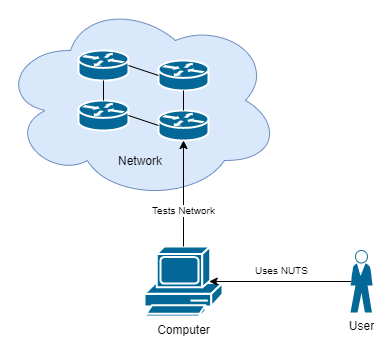
\includegraphics[scale=0.7]{\vorlagenOrdner/Bilder/SystemUebersicht}

	\subsection{Computer}
		Dies entspricht unserem Client.
		Auf dem Computer läuft das zu entwickelnde System, welches aus einem Python Programm besteht und mittels Nornir mit einem Netzwerk kommuniziert und Tests darauf ausführt.

	\subsection{Netzwerk}
		Dies ist das Netzwerk, auf dem die automatisierten Tests ausgeführt werden sollen. 
		Es besteht aus mehreren Netzwerkknoten, z.B. Switches, Router und Clients.
		Das Netzwerk wird über eine lokale Schnittstelle oder über das Internet angesteuert.

	\subsection{Datenablage}
		Die Datenablage befindet sich auf dem Computer und kann bei Bedarf über ein Verwaltungstool mit anderen Clients geteilt werden. 
		Darin befinden sich sämtliche für das Testsystem benötigte Daten.
		Diese Daten werden in Form von YAML-Files als Key-Value Store angelegt.

\section{Deployment}
	\subsection{Deploymentdiagramm}
		\includegraphics[scale=0.7]{\vorlagenOrdner/Bilder/Deploymentdiagramm}
	
		\subsection{Client}
		Der User Client kann ein Computer oder ein Server sein, welcher die automatisierten Tests ausführen soll.
		Darauf läuft ein beliebiges Betriebssystem

		\subsection{Betriebssystem}
		Es gibt keine spezifischen Anforderungen an das Betriebssystem, welches auf dem Client installiert ist.
		Python Code lässt sich auf beliebigen Betriebssystemen ausführen.

		\subsection{Python Installation}
		Für die Ausführung von Python-Code muss Python auf dem Client installiert sein. 

		\subsection{NUTS2.0}
		Das zu entwickelnde Programm, welches auf dem Client installiert wird. 
		Es verbindet sich mit einem Netzwerk und führt vorher definierte Tests darauf aus.

\section{Ausbauszenarien}
	\subsection{Szenario 1: Erweiterung um weitere Neztwerktests}
	Die Erweiterung des Systems um weitere Tests wird durch die Architektur so einfach wie möglich gehalten.
	Es müssen lediglich die Testfactory angepasst und neue Testklassen erstellt werden, um neue Tests durch das System zu ermöglichen.
	Die Tests können danach in der Testdefinition angelegt werden.

	\subsection{Szenario 2: Erweiterung um Netzwerkschnittstellen}
	Durch den Einsatz des Factory- und Strategy-Pattern wird die Erweiterung um neue Schnittstellen vereinfacht.
	Die Factory muss um die neue Schnittstelle erweitert und die Schnittstelle als Klasse implementiert werden.
	Danach sollte sich die Schnittstelle über die Testdefinition aufrufen lassen.

	\subsection{Szenario 3: Erweiterung um eine Graphische Benutzeroberfläche (GUI)}
	Das System wird mit einem Fokus auf die Funktionalität entwickelt.
	Dabei wird die Usability durch die Verwendung eines GUI vorerst vernachlässigt.
	Die Erfassung von Netzwerkgeräten, das Erfassen von Tests und die Orchestrierung der Tests liessen sich alle über eine Benutzeroberfläche ansteuern.
	Nach der Einschätzung der Autoren entspricht die GUI-Erweiterung ungefähr drei bis sechs Wochen Arbeit.
	Es ist darauf zu achten, die Prinzipien der nutzerzentrierten Entwicklung (User Centered Design) anzuwenden und regelmässig Usability-Tests durchzuführen.

	\subsection{Szenario 4: Anbindung einer Datenbank}
	Eine Datenbank würde dem System diverse Möglichkeiten für die effizientere Datenhaltung ermöglichen:
	\begin{itemize}
		\item Geräte liessen sich in einer Graphdatenbank mit den jeweiligen Verbindungen als Relationen speichern, was eine intuitive Darstellung und effiziente Abfragen ermöglicht.
		\item Durch die Verwendung einer Datenbank liessen sich das Inventar und die Testdefinitionen einfacher von mehreren Clients verwenden und untereinander austauschen.
		\item Passwörter von Devices, welche nach der aktuellen Architektur in Plaintext gespeichert werden, wären in einer Datenbank besser gesichert.
	\end{itemize}
	Auch hier ist mit Aufwand von drei bis vier Wochen zu rechnen. 
	Ausserdem wird für die Haltung einer Datenbank Hardware, beispielsweise ein DB-Server, benötigt.
	
	\subsection{Szenario 5: Erweiterung um Security}
	Damit Passwörter nicht in Plaintext gespeichert werden und von potentiellen Angreifern einfach ausgelesen werden können,
	benötigt das System eine  Verschlüsselung der Konfigurationsdaten. 
	Am einfachsten lässt sich dies erreichen, wenn sich der Benutzer gegenüber der Softwar mit einem Passwort authentifizieren muss, um zugriff auf die Konfigruation zu erhalten.
	Dafür müsste der Python-Code mit einer Security-Library erweitert werden und der Code müsste angepasst werden.
	Deviceinformationen würden dann nur noch in Encrypteter Form gespeichert werden.

	Bei dieser Erweiterung ist darauf zu achten, dass das System so robust wie möglich bleibt.
	Beispielsweise müssen im falle eines Fehlers sämtliche Konfigurationen der Devices wieder Verschlüsselt werden, bevor sie gespeichert werden.
	

	

\end{document}